\documentclass[a4paper]{oblivoir}
\usepackage{amsmath,amssymb,kotex,kswrapfig,mdframed,paralist}
\usepackage{fapapersize}
\usefapapersize{210mm,297mm,20mm,*,20mm,*}

\usepackage{tabto,pifont}
\TabPositions{0.2\textwidth,0.4\textwidth,0.6\textwidth,0.8\textwidth}
\newcommand\tabb[5]{\par\noindent
\ding{172}\:{\ensuremath{#1}}
\tab\ding{173}\:\:{\ensuremath{#2}}
\tab\ding{174}\:\:{\ensuremath{#3}}
\tab\ding{175}\:\:{\ensuremath{#4}}
\tab\ding{176}\:\:{\ensuremath{#5}}}

\usepackage{graphicx}

%\pagestyle{empty}

%%% Counters
\newcounter{num}

%%% Commands
\newcommand\prob[1]
{\bigskip\bigskip\par\noindent\stepcounter{num} \textbf{문제 \thenum) #1}\par\noindent}

\newcommand\pb[1]{\ensuremath{\fbox{\phantom{#1}}}}

\newcommand\ba{\ensuremath{\:|\:}}

\newcommand\vs[1]{\vspace{25pt}}

\newcommand\an[1]{\bigskip\par\noindent\textbf{문제 #1)}\par\noindent}

%%% Meta Commands
\let\oldsection\section
\renewcommand\section{\clearpage\oldsection}

\let\emph\textsf

\begin{document}
\begin{center}
\LARGE준영, 미니테스트 16
\end{center}
\begin{flushright}
날짜 : 2017년 \(\pb3\)월 \(\pb{10}\)일 \(\pb{월}\)요일
,\qquad
제한시간 : \pb{17년}분
,\qquad
점수 : \pb{20} / \pb{20}
\end{flushright}

%
\prob{}
미분가능한 함수 \(f(x)\)에 대하여 \(f'(a)=-3\)이고,
\(\displaystyle\lim_{h\to0}\frac{f(a-2h)-f(a+h)+g(h)}h=2\)일 때,
\(\displaystyle\lim_{h\to0}\frac{g(h)}h\)의 값을 구하여라.

%
\prob{}
함수 \(f(x)\)에 대하여 \(f'(2)=3\)일 때, \(\displaystyle\lim_{x\to2}\frac{x^3-8}{f(x)-f(2)}\)의 값을 구하여라.

%
\prob{}
함수 \(f(x)\)에 대하여 \(f(2)=3\), \(f'(2)=1\)일 때, \(\displaystyle\lim_{x\to2}\frac{2f(x)-xf(2)}{x-2}\)의 값을 구하여라.

%
\prob{}
함수 \(f(x)\)에 대하여 \(f(1)=2\), \(f'(1)=4\)일 때, \(\displaystyle\lim_{x\to1}\frac{x^2f(1)-f(x^2)}{x-1}\)의 값을 구하여라.

%
\prob{}
\begin{minipage}{0.45\textwidth}
함수 \(y=f(x)\)의 그래프가 오른쪽 그래프와 같을 때, 다음 <보기>중 옳은 것을 골라라.
\end{minipage}
\begin{minipage}{0.45\textwidth}\centering
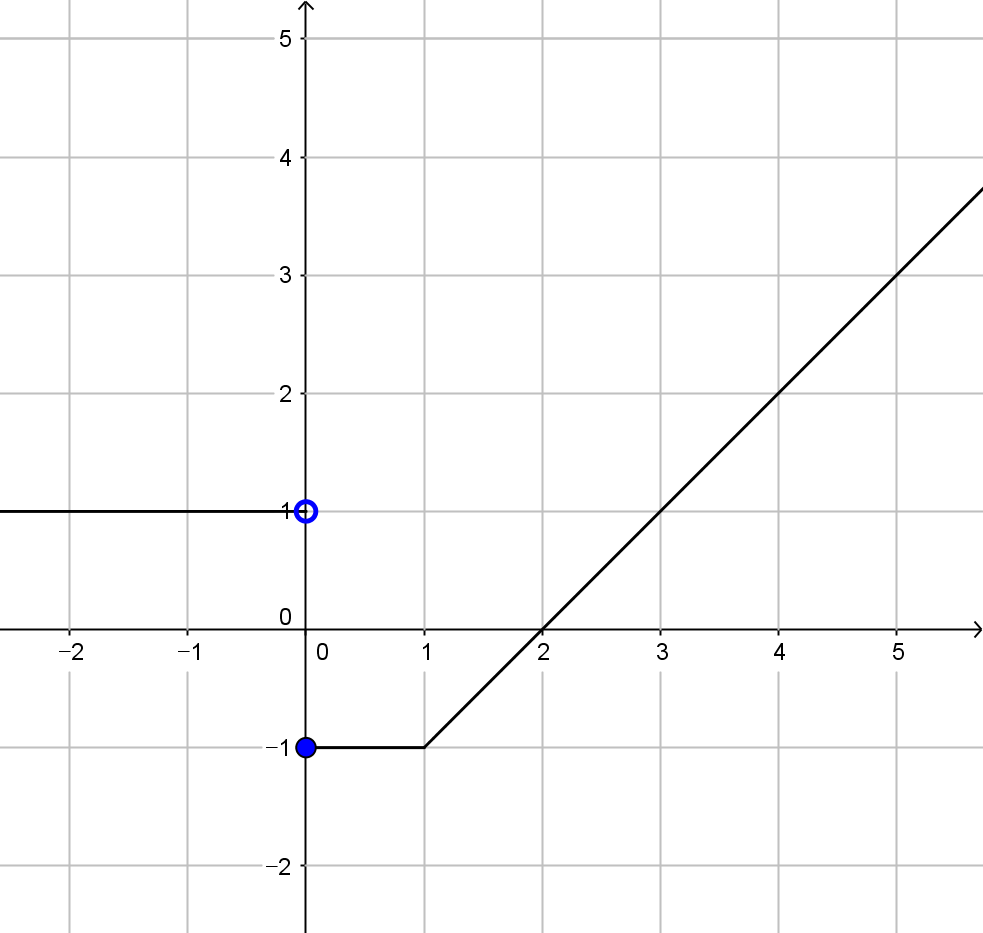
\includegraphics[width=0.45\textwidth]{continuity_test}
\end{minipage}

\begin{mdframed}[frametitle=<보기>]
\begin{enumerate}
\item[ㄱ.]
\(f(x)\)는 \(x=1\)에서 미분가능하다.
\item[ㄴ.]
\(xf(x)\)는 \(x=0\)에서 미분가능하다.
\item[ㄷ.]
\(x^2f(x)\)는 \(x=0\)에서 미분가능하다.
\end{enumerate}
\end{mdframed}

%
\prob{}
함수 \(f(x)=(x+2)(x^2-3x+4\)에 대하여 \(f'(1)\)의 값을 구하여라.

%
\prob{}
함수 \(f(x)=5x^4+x^3-3x-8\)에 대하여 \(f'(1)\)의 값을 구하여라.

%
\prob{}
함수 \(f(x)=(x+1)(2x+3)(3x-1)\)에 대하여 \(f'(0)\)의 값을 구하여라.

\clearpage
%
\prob{}
함수 \(f(x)=(x+1)^3(x^2-1)^2\)에 대하여 \(f'(0)\)의 값을 구하여라.

%
\prob{}
함수 \(f(x)=ax^2+bx+c\)에서 \(f(0)=5\), \(f'(1)=-4\), \(f'(-1)=8\)을 만족시킬 때, 상수 \(a\), \(b\), \(c\)의 값을 각각 구하여라.

%
\prob{}
함수 \(f(x)=3x^2+ax+1\)의 그래프 위의 점 \((1,7)\)에서의 접선의 기울기가 \(m\)일 때, 상수 \(a\), \(m\)의 곱 \(am\)의 값을 구하여라.

%
\prob{}
\(f(x)=x^4-2x^3+x+4\)일 때, \(\displaystyle\lim_{h\to0}\frac{f(1+h)-f(1-h)}h\)의 값을 구하여라.

%
\prob{}
\(\displaystyle\lim_{x\to1}\frac{x^{10}+x-2}{x-1}\)의 값을 구하여라.

%
\prob{}
함수 \(f(x)=\begin{cases}a(x-4)^2+b&(x\ge2)\\x^2&(x<2)\end{cases}\)이 \(x=2\)에서 미분가능할 때, 상수 \(a\), \(b\)의 값을 각각 구하여라.

%
\prob{}
함수 \(f(x)=\begin{cases}x^3+ax^2+bx&(x\ge1)\\2x^2+1&(x<1)\end{cases}\)이 모든 실수 \(x\)에서 미분가능할 때, 상수 \(a\), \(b\)의 곱 \(ab\)의 값을 각각 구하여라.

%
\prob{}
다항식 \(x^{100}-2x^3+4\)를 \((x-1)^2\)으로 나누었을 때의 나머지를 구하여라.

%
\prob{}
함수 \(f(x)\)가 \(x\)에 대한 다항식이고 \(f(1)=2\), \(f'(1)=3\)일 때, \(f(x)\)를 \((x-1)^2\)으로 나누었을 때의 나머지를 구하여라.

%
\prob{}
다음 곡선 위의 주어진 점에서의 접선의 기울기를 구하여라.
\begin{enumerate}[(1)]
\item
\(y=2x^2+4x-3\quad(1,3)\)
\item
\(y=x^3-2x+1\quad(2,5)\)
\end{enumerate}

\clearpage
%
\prob{}
곡선 \(f(x)=ax^3+bx^2+cx\) 위의 두 점 \((1,3)\), \((2,0)\)에서의 접선의 기울기가 같을 때, 상수 \(a\), \(b\), \(c\)의 값을 각각 구하여라.

%
\prob{}
곡선 \(y=x^3+2x^2+x-2\)에 대하여 다음을 구하여라.
\begin{enumerate}[(1)]
\item
곡선 위의 점 \((1,2)\)에서의 접선의 방정식
\item
곡선 위의 점 \((1,2)\)를 지나고 이 점에서의 접선에 수직인 직선의 방정식
\end{enumerate}

%
\prob{}
곡선 \(y=x^2-3x\)에 대하여 다음과 같은 접선의 방정식을 구하여라.
\begin{enumerate}[(1)]
\item
\(x\)축에 평행한 직선
\item
기울기가 \(3\)인 접선
\end{enumerate}

%
\prob{}
직선 \(x+9y=3\)에 수직이고 곡선 \(y=x^3+3x^2+2\)에 접하는 직선의 방정식을 구하여라.

%
\prob{}
점 \((0,-4)\)에서 곡선 \(y=x^2-2x\)에 그은 접선의 방정식을 구하여라.

\end{document}